% 1977 年河南卷第五题：正方形 ABCD（A 左上、D 右上、B 左下、C 右下），
% E 在 DC 边上，F 在 BC 延长线上（CF=CE），BE 与 DF 交于 G（按源卷第 2 页布局）
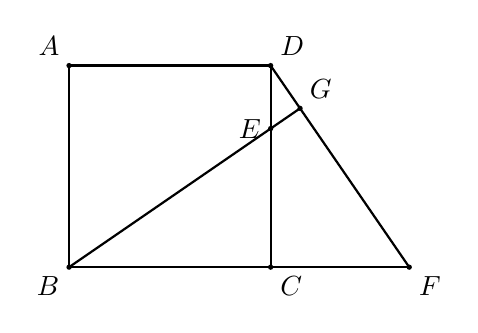
\begin{tikzpicture}[scale=0.8]
  \coordinate (A) at (0,3.2);
  \coordinate (D) at (3.2,3.2);
  \coordinate (C) at (3.2,0);
  \coordinate (B) at (0,0);
  \coordinate (E) at (3.2,2.2);
  \coordinate (F) at (5.4,0);
  \coordinate (G) at (3.667,2.521);
  \draw[thick] (A)--(D)--(C)--(B)--cycle;
  \draw[thick] (C)--(F);
  \draw[thick] (B)--(G);
  \draw[thick] (D)--(F);
  \fill (A) circle (1.2pt) node[above left] {$A$};
  \fill (D) circle (1.2pt) node[above right] {$D$};
  \fill (C) circle (1.2pt) node[below right] {$C$};
  \fill (B) circle (1.2pt) node[below left] {$B$};
  \fill (E) circle (1.2pt) node[left] {$E$};
  \fill (F) circle (1.2pt) node[below right] {$F$};
  \fill (G) circle (1.2pt) node[above right] {$G$};
\end{tikzpicture}
